\section{Coordination}

\begin{multicols}{2}


\section*{The Nervous System}


\subsection{Nerve Model} % VSO 48

\begin{center}
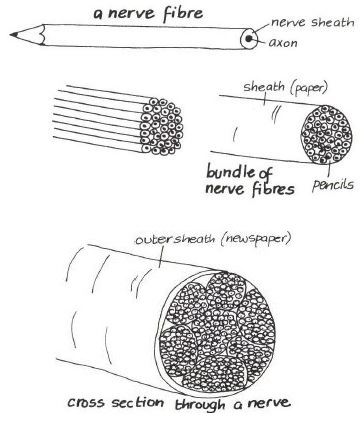
\includegraphics[width=0.45\textwidth]{./img/vso/nerve-model.jpg}
\end{center}

\begin{description*}
%\item[Subtopic:]{}
\item[Materials:]{Pencils, paper, newspaper}
%\item[Setup:]{}
\item[Procedure:]{Use a pencil to represent a nerve fibre. Roll many pencils in a sheet of paper to represent a bundle of fibres. Roll many bundles in a newspaper to represent a nerve.}
%\item[Hazards:]{}
%\item[Questions:]{}
%\item[Observations:]{}
%\item[Theory:]{}
%\item[Applications:]{}
\item[Notes:]{Use sticks, straws or grasses as substitutes for pencils.}
\end{description*}

\subsection{Neuron Models}

\begin{center}
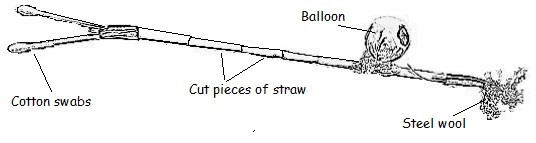
\includegraphics[width=0.49\textwidth]{./img/neuron-model.jpg}
\end{center}

\begin{description*}
%\item[Subtopic:]{}
\item[Materials:]{Straight stick/bamboo skewer, straws, tape, balloon, steel wool, cotton swabs, scissors}
%\item[Setup:]{}
\item[Procedure:]{Cut several short lengths of straw and place them over a bamboo skewer or straight stick. Fill a balloon slightly and tape it a few centimetres from one end. Draw a large black dot on the balloon. Attach steel wool and cotton swabs to the ends as shown.}
%\item[Hazards:]{}
%\item[Questions:]{}
%\item[Observations:]{}
%\item[Theory:]{}
%\item[Applications:]{}
\item[Notes:]{Use similar materials to make models of other types of neurons.}
\end{description*}

%==================================================================================================%

\section*{Reflex Actions}


\subsection{Light in the Eye}

\begin{center}
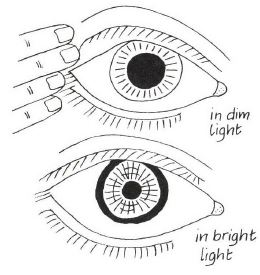
\includegraphics[width=0.25\textwidth]{./img/vso/light-eye.jpg}
\end{center}

\begin{description*}
%\item[Subtopic:]{}
%\item[Materials:]{}
%\item[Setup:]{}
\item[Procedure:]{Cover one eye and look into a
bright light. After the uncovered
eye has adjusted to the light
uncover the other eye. Quickly
compare the sizes of the pupils in
each eye.}
%\item[Hazards:]{}
%\item[Questions:]{}
%\item[Observations:]{}
\item[Theory:]{The size of the pupil is
adjusted by a reflex action. In
bright light the circular muscles of
the iris diaphragm contract and
the pupil becomes smaller.}
%\item[Applications:]{}
%\item[Notes:]{}
\end{description*}

\subsection{Blinking Reflex}

\begin{center}
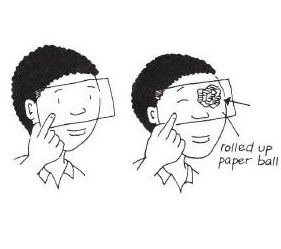
\includegraphics[width=0.4\textwidth]{./img/vso/blinking.jpg}
\end{center}

\begin{description*}
%\item[Subtopic:]{}
\item[Materials:]{Plastic sheet, paper ball}
%\item[Setup:]{}
\item[Procedure:]{One student holds a clear piece of
plastic to protect his or her eyes.
The plastic from a large plastic
bottle is suitable. Another student
throws a crumpled ball of paper
at the plastic. }
%\item[Hazards:]{}
%\item[Questions:]{}
\item[Observations:]{The first student
blinks. Blinking is a reflex
reaction.}
%\item[Theory:]{}
%\item[Applications:]{}
%\item[Notes:]{}
\end{description*}

\subsection{Knee Jerk}

\begin{center}
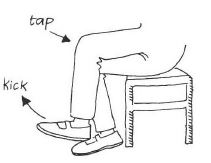
\includegraphics[width=0.4\textwidth]{./img/vso/knee-jerk.jpg}
\end{center}

\begin{description*}
%\item[Subtopic:]{}
%\item[Materials:]{}
%\item[Setup:]{}
\item[Procedure:]{Cross one leg over the other. Tap
just below the knee cap as shown.
}
%\item[Hazards:]{}
%\item[Questions:]{}
\item[Observations:]{The tapped leg kicks up in an
involuntary reflex response.}
%\item[Theory:]{}
%\item[Applications:]{}
%\item[Notes:]{}
\end{description*}

%==================================================================================================%

\section*{Sense Organs}


\subsection{Taste Map}

\begin{center}
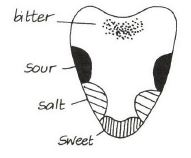
\includegraphics[width=0.35\textwidth]{./img/vso/taste-map.jpg}
\end{center}

\begin{description*}
%\item[Subtopic:]{}
\item[Materials:]{4 glasses, spoon, coffee, vinegar, salt, sugar, water}
\item[Setup:]{Prepare the 4 taste solutions as follows:
\begin{itemize}
\item Bitter: Lemon peel, coffee dissolved in water or strong cold tea
\item Sour:Vinegar or lime juice
\item Salty: Salt dissolved in water
\item Sweet: Sugar dissolved in water
\end{itemize}}
%\item[Bitter:]{Lemon peel, coffee dissolved in water or strong cold tea}
%\item[Sour:]{Vinegar or lime juice}
%\item[Salty:]{Salt dissolved in water}
%\item[Sweet:]{Sugar dissolved in water}
\item[Procedure:]{Use a spoon to pour a small amount of each solution in students' hands, one at a time. Have them taste the solution and describe the taste, as well as where on their tongues the taste in found.}
%\item[Questions:]{}
%\item[Observations:]{}
\item[Theory:]{The tongue has receptors for different tastes in different places. Make a diagram of the tongue as shown to display in the class.}
%\item[Applications:]{}
%\item[Notes:]{}
\end{description*}

\subsection{Tasteless Food}

%\begin{center}
%\includegraphics[width=0.4\textwidth]{./img/.jpg}
%\end{center}

\begin{description*}
%\item[Subtopic:]{}
\item[Materials:]{Onion, apple or other fruit}
%\item[Setup:]{}
\item[Procedure:]{Cut an onion and an apple into small pieces. Blindfold the person to be
tested and make them hold their nose.}
%\item[Hazards:]{}
%\item[Questions:]{}
\item[Observations:]{They will find the apple and
onion taste the same! If students can detect the difference, try giving
them the smell of onion as they eat the apple!}
\item[Theory:]{Smell is very important
in identifying foods. A cold or a blocked nose makes it difficult to taste
properly.}
%\item[Applications:]{}
%\item[Notes:]{}
\end{description*}

\subsection{Sound and Direction}

\begin{center}
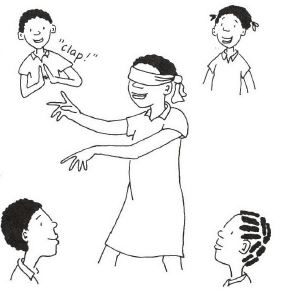
\includegraphics[width=0.4\textwidth]{./img/vso/sound-direction.jpg}
\end{center}

\begin{description*}
%\item[Subtopic:]{}
\item[Materials:]{Cloth/kanga}
%\item[Setup:]{}
\item[Procedure:]{One student is blindfolded and
stands in a circle made by the
others. One at a time each person
in the circle makes a small noise.
At each noise the blindfolded
student points to the direction of
the sound.}
%\item[Hazards:]{}
\item[Questions:]{How accurately can students
detect the direction of the sound?}
%\item[Observations:]{}
%\item[Theory:]{}
%\item[Applications:]{}
\item[Notes:]{Cover one ear (with cotton wool
or a cloth).}
\end{description*}

\subsection{Sight and Balance}

\begin{center}
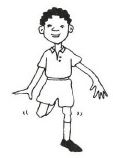
\includegraphics[width=0.25\textwidth]{./img/vso/sight-balance.jpg}
\end{center}

\begin{description*}
%\item[Subtopic:]{}
%\item[Materials:]{}
%\item[Setup:]{}
\item[Procedure:]{Try balancing on one leg with
both eyes closed. Now try with
the eyes open. }
%\item[Hazards:]{}
%\item[Questions:]{}
\item[Observations:]{It is easier to
balance with the eyes open -
sight is an aid to balance.}
%\item[Theory:]{}
\item[Applications:]{Ask students to spin round and
discuss whether it is easier to
regain balance when the eyes are
open.}
%\item[Notes:]{}
\end{description*}

%==================================================================================================%

\section*{Coordination in Plants}


\subsection{Phototropism}

\begin{center}
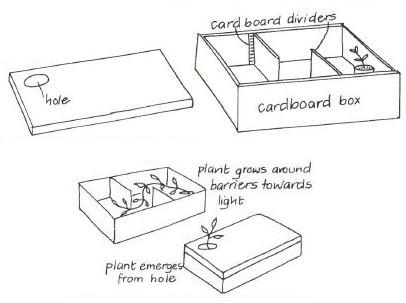
\includegraphics[width=0.45\textwidth]{./img/vso/phototropism.jpg}
\end{center}

\begin{description*}
%\item[Subtopic:]{}
\item[Materials:]{Cardboard box, seedlings in small pots}
%\item[Setup:]{}
\item[Procedure:]{Make a light maze box as shown. Lift the lid daily to watch progress.}
%\item[Hazards:]{}
%\item[Questions:]{}
%\item[Observations:]{}
%\item[Theory:]{}
\item[Applications:]{Farmers and gardeners see leaves turning to the Sun after disturbance
or transplanting. Place a house plant next to a window letting in
sunlight. Leave it for a few days. Now rotate the pot and note the
position of the leaves. Examine the plant over the next few days. The
leaves turn towards the light as the plant grows.}
%\item[Notes:]{}
\end{description*}

\subsection{Geotropism - Shoots}

\begin{center}
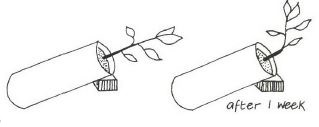
\includegraphics[width=0.4\textwidth]{./img/vso/geotropism-shoots.jpg}
\end{center}

\begin{description*}
%\item[Subtopic:]{}
%\item[Materials:]{}
%\item[Setup:]{}
\item[Procedure:]{Lean a pot plant at an angle.
Leave it for a week. Notice that
after this time the leaves turn
upwards.}
%\item[Hazards:]{}
%\item[Questions:]{}
%\item[Observations:]{}
%\item[Theory:]{}
%\item[Applications:]{}
%\item[Notes:]{}
\end{description*}

\subsection{Geotropism - Roots}

\begin{center}
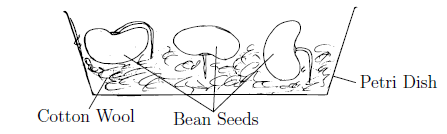
\includegraphics[width=0.45\textwidth]{./img/geotropism.png}
\end{center}

\begin{description*}
%\item[Subtopic:]{}
\item[Materials:]{Cotton wool, bean seeds, plastic bottle}
%\item[Setup:]{}
\item[Procedure:]{Cut the bottom of a plastic bottle to act as a petri dish. Place damp cotton wool at the bottom and a few bean seeds on top.}
%\item[Hazards:]{}
%\item[Questions:]{}
\item[Observations:]{Plant roots will grow towards gravity, showing positive geotropism.
The stems will grow away from gravity, thus showing negative geotropism.}
%\item[Theory:]{}
%\item[Applications:]{}
%\item[Notes:]{}
\end{description*}

\subsection{Hydrotropism}

\begin{center}
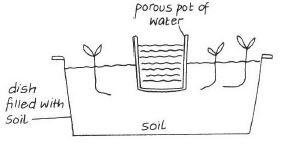
\includegraphics[width=0.4\textwidth]{./img/vso/hydrotropism.jpg}
\end{center}

\begin{description*}
%\item[Subtopic:]{}
\item[Materials:]{Large dish, porous pot, soil, water, seedlings}
%\item[Setup:]{}
\item[Procedure:]{Fill the porous pot with water as shown.}
%\item[Hazards:]{}
%\item[Questions:]{}
\item[Observations:]{The seedlings' roots will grow
towards the porous pot (source of water).}
%\item[Theory:]{}
%\item[Applications:]{}
%\item[Notes:]{}
\end{description*}

\subsection{Hothouses}

\begin{center}
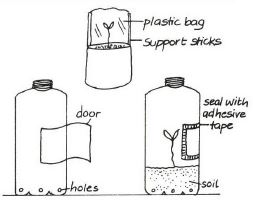
\includegraphics[width=0.4\textwidth]{./img/vso/hothouses.jpg}
\end{center}

\begin{description*}
%\item[Subtopic:]{}
\item[Materials:]{Plastic bags, wire/stick supports, plastic bottles}
%\item[Setup:]{}
\item[Procedure:]{Use plastic bags supported by
sticks or wire to form a hothouse
over any container. Or cut a door in a plastic bottle and
plant seeds inside the mini-hothouse.}
%\item[Hazards:]{}
%\item[Questions:]{}
%\item[Observations:]{}
\item[Theory:]{Hothouses are warmer than the
outside air and so crops, such as
lettuce or tomatoes will grow
faster.}
%\item[Applications:]{}
%\item[Notes:]{}
\end{description*}

%==================================================================================================%


\end{multicols}

\pagebreak